\pdfoutput=1
\documentclass[a0,portrait,25pt]{sciposter}

% Служи за оформяне на текста в колони.
\usepackage{multicol}

% Задава разстоянието между колоните в постера.
\columnsep=20pt

% Задава дебелината на линията разделяща колоните в постера.
\columnseprule=1pt

% Задава цветове според техните SVG названия. Пълният списък с цветовете е наличен на: http://www.latextemplates.com/svgnames-colors
\usepackage[svgnames]{xcolor}

% Използване на Times шрифтовете.
\usepackage{times}

% Използва се за включването на изображения.
\usepackage{graphicx}
\graphicspath{{images/}}

% Позволява промяна на фоновия цвят. 
\usepackage{pagecolor}

% Позволява използването на текст в кутии и фонов цвят.
\usepackage{mdframed}

\begin{document}

% Фонов цвят на постера.
\pagecolor{LightGray}

\begin{mdframed}[backgroundcolor=white,roundcorner=4pt,shadow=true,linewidth=1pt]
\begin{minipage}[b]{1.44  \linewidth}
\begin{multicols}{2}
\
\color{DimGray}
\Huge \textbf{Slot Machine Reels Reconstruction \\ with Genetic Algorithms} \\
% Имена на авторите.
\huge {Petar Tomov, Iliyan Zankinski, Todor Balabanov} \\ [0.5cm] 
% Название на института.
\huge Institute of Information and Communication Technologies \\  Bulgarian Academy of Sciences \\ [0.4cm]
% Електронен адрес за връзка.
\Large \texttt{todorb@iinf.bas.bg}


\includegraphics[width=20cm]{logo-iict-en}
\end{multicols}
\end{minipage}
\end{mdframed}

% Разстояние между заглавната част на постера и същинското изложение. 
\vspace{0.5cm}

% Въведение. 
\begin{mdframed}[backgroundcolor=white,roundcorner=4pt,shadow=true,linewidth=1pt]
\color{Black}
\section*{Introduction}
This research focuses on a very well know problem in the slot machine gambling games development - reverse engineering of the virtual reels. Virtual reels are trade secretes of the manufacturer usually. They are a discrete random distribution of the game symbols. The value for return to player (RTP) is adjusted by the placement of the symbols. If the RTP needs to be checked (without access to the game source code) a reconstruction of the virtual reels is necessary. Such check starts with visual observation of the game screens or by image processing of game screen-shots. This research proposes Genetic Algorithm (GA) as search technique for slot machines virtual reels reconstruction.
\end{mdframed}

% Разделя постера в три колони.
\begin{multicols}{3}

% Обяснение какво представляват барабаните на една хазртна игра от тип ротативка.
\begin{mdframed}[backgroundcolor=white,roundcorner=4pt,shadow=true,linewidth=1pt]
\color{Black}
\section*{Slot Machine Reels}
For better understanding of the problem a brief description of the slot machine reels will be given. One of the basic concepts of the slots are the spinning reels. In the beginning slots were mechanical. Reels were driven to spin by manual handle. Nowadays slots are generally computerized. It means that mechanical reels are replaced with virtual reels. 
\end{mdframed}

% Екран на слот машина.
\begin{mdframed}[backgroundcolor=white,roundcorner=4pt,shadow=true,linewidth=1pt]
\section*{Slot Machine Screens}
\begin{minipage}[c]{1\linewidth}
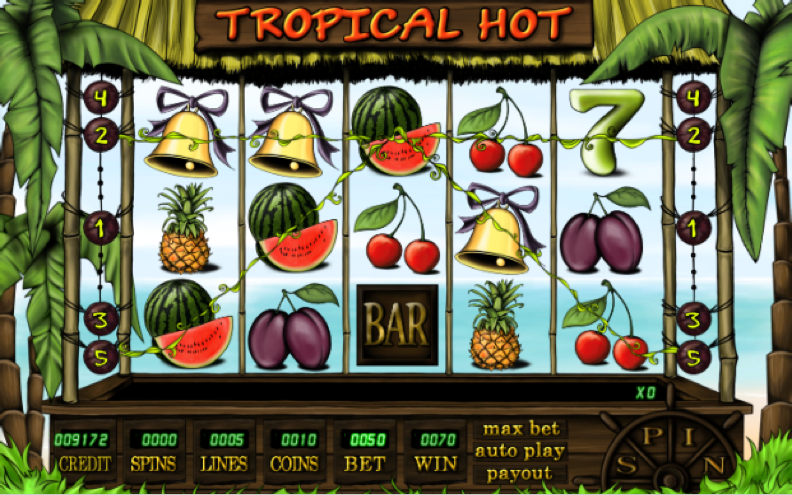
\includegraphics[width=0.9\linewidth]{pic003} \\

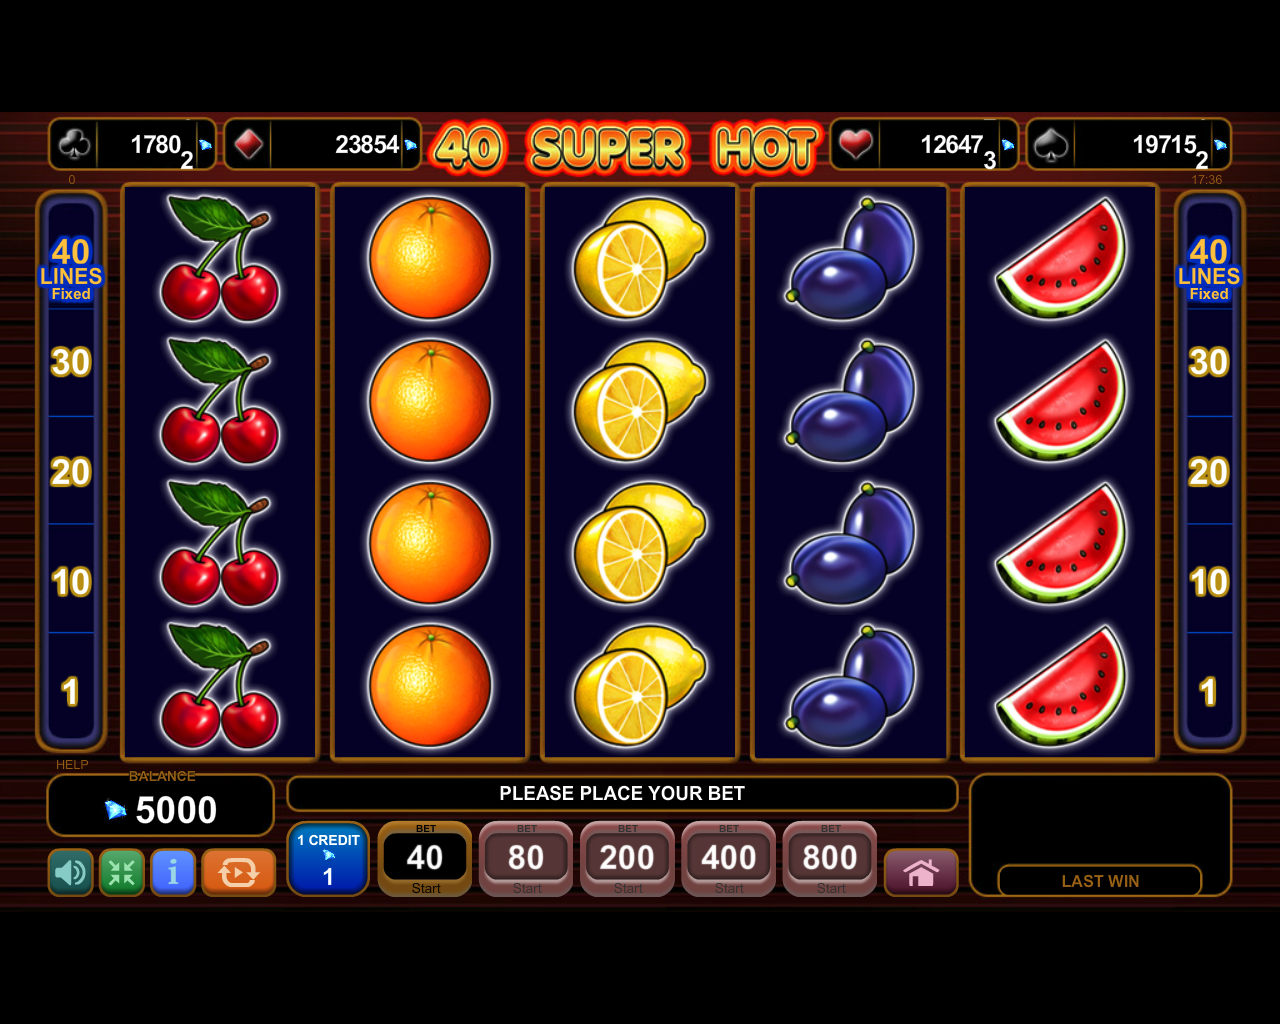
\includegraphics[width=0.9\linewidth]{pic004} \\
\end{minipage}
\end{mdframed}

% Обяснение за генераторите на псевдо-случайни числа.
\begin{mdframed}[backgroundcolor=white,roundcorner=4pt,shadow=true,linewidth=1pt]
\color{Black}
\section*{Pseudorandom Number Generators}
There is no handle anymore, but a button and a pseudo-random number generator (PRNG) are used for the outcome. Win is calculated according to symbols patterns that appear on the screen after the reels have stopped spinning. A known pay table defines how valuable each symbol on the screen is. More frequent symbols are less profitable and less frequent symbols are much more profitable and informative for reels reconstruction process. 
\end{mdframed}

% Обяснение за процента върнат към играча.
\begin{mdframed}[backgroundcolor=white,roundcorner=4pt,shadow=true,linewidth=1pt]
\color{Black}
\section*{Return to Player}
The accuracy of game RTP is used to measure reels reconstruction quality. If the reconstruction is good enough the RTP will be close to the RTP published by the manufacturer. When the game is produced the desired RTP is adjusted by mathematicians and game designers. Their job is to populate game reels with proper symbols in proper discrete distribution. The process of reels reconstruction is pretty similar to the process of the new reels construction. The only difference is about symbols classification patterns and the requirement this patterns to be presented in the reconstructed reels.
\end{mdframed}

% Таблица на печалбите.
\begin{mdframed}[backgroundcolor=white,roundcorner=4pt,shadow=true,linewidth=1pt]
\section*{Slot Machine Paytable}
\begin{minipage}[c]{1\linewidth}
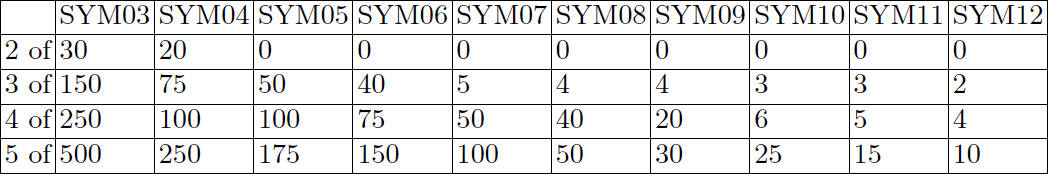
\includegraphics[width=1.0\linewidth]{pic002}
\end{minipage}
\end{mdframed}

% Линии на залози.
\begin{mdframed}[backgroundcolor=white,roundcorner=4pt,shadow=true,linewidth=1pt]
\section*{Slot Machine Betting Lines}
\begin{minipage}[c]{1\linewidth}
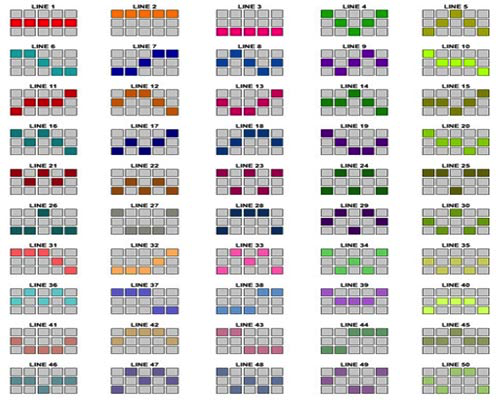
\includegraphics[width=0.9\linewidth]{pic001}
\end{minipage}
\end{mdframed}

\begin{mdframed}[backgroundcolor=white,roundcorner=4pt,shadow=true,linewidth=1pt]
\color{Black}
\section*{Image Processing of Slot Screens}
Virtual reels analysis starts with screen pattern classification as image processing ( http://github.com/ TodorBalabanov/Slot-Machine-Symbols-Capture ). Classified patterns are used as pieces in the reconstructed sequence of the reels. A list of the classified patterns is the input for the algorithm ( http://github.com/ TodorBalabanov/Slot-Machine-Reel-Mosaicing ). 
\end{mdframed}

\begin{mdframed}[backgroundcolor=white,roundcorner=4pt,shadow=true,linewidth=1pt]
\color{Black}
\section*{Genetic Algorithms}
The software implementation uses Apache Commons Genetic Algorithms Framework. Chromosomes are characters sequences of the symbols available in the slot game. The crossover operator is chosen to be a single cut point. It is the preferred way because strips of the symbols should be kept as much in order as possible. Crossover rate is experimentally chosen to be 90\%. Mutation operator is done in the simplest possible way by swapping two symbols in a single reel. Mutation rate is experimentally chosen to be 10\%. Tournament selection with arity value of 2 is used for reproducing parents choosing. Population of 23 individuals is selected experimentally. Reels reconstruction problem is highly combinatorial and because of this maximum running time is chosen as optimization stopping criteria. When the problem is highly combinatorial it is useful to apply elitism rule as it is applied in this research with rate of 10\%. The most complex part in the solution proposed is the fitness function organization. 
\end{mdframed}

\begin{mdframed}[backgroundcolor=white,roundcorner=4pt,shadow=true,linewidth=1pt]
\color{Black}
\section*{Fintess Function}
Five different components were involved in fitness function composition: \\

1) Number of wrong patterns found in the reconstructed reel, but not presented in classified patterns; 

2) Number of missing patterns which should be presented in the reconstructed reel, because they are presented in the classified patterns; 

3) Number of patterns which repeats more than once in the reconstructed reel; 

4) Length of the reconstructed reel; 

5) Euclidean distance of symbols frequencies between reconstructed reel and classified patterns. \\

These five components can be separated in two groups of constraints: First and second are hard constraints (should not be violated) and the other three are soft constraints (can be violated). \\
\end{mdframed}

\begin{mdframed}[backgroundcolor=white,roundcorner=4pt,shadow=true,linewidth=1pt]
\color{Black}
\section*{Important Criterias}
The most important criteria is related to wrong patterns. If in the reconstructed reel there are unobserved patterns it means that the reconstructed reel is generally wrong and the desired RTP will not be achieved. Secondly most important criteria is related to the missing patterns. If the patterns were observed, but they are missing in the reconstructed reel it means that the reel is not close enough to the original reel. Repeating patterns (third constraint) are not desirable, because they extend the length of the reconstructed reel, but can be accepted. Reconstructed reels are better accepted when they are as short as possible (fourth constraint), but length can vary. The final constraint is about the Euclidean closeness between the reconstructed reel and the classified patterns. 
\end{mdframed}

\begin{mdframed}[backgroundcolor=white,roundcorner=4pt,shadow=true,linewidth=1pt]
\color{Black}
\section*{Symbols Frequencies Closeness}
Symbols frequencies are calculated for the classified patterns in the beginning of the algorithm. At each fitness function calculation symbols frequencies are calculated for each reconstructed reel. The reconstructed reel gets closer to the real reel when symbol frequencies are close. 
\end{mdframed}

\begin{mdframed}[backgroundcolor=white,roundcorner=4pt,shadow=true,linewidth=1pt]
\color{Black}
\section*{Conclustions}
Experiments show that absolutely automatic reconstruction is not possible with GA technique, but with some manual adjustments reconstructed reels are close to originals at least as RTP achieved. As further research it will be interesting reconstruction approach to be extended to optimization with Context-Sensitive Grammars (CSG).
\end{mdframed}

% Секция за служебна информация.
\begin{mdframed}[backgroundcolor=white,roundcorner=4pt,shadow=true,linewidth=1pt]
\color{Black}
% Биглиография.
\section*{References}
\begin{enumerate}
\item P. Tomov, I. Zankinski, T. Balabanov, \textit{Slot Machine Reels Reconstruction with Monte-Carlo Search}, International Scientific Conference UniTech, 2017.
\item D. Keremedchiev, P. Tomov, M. Barova, \textit{Slot Machine Base Game Evolutionary RTP Optimization}, International Conference on Numerical Analysis and Its Applications, 2017.
\item T. Balabanov, I. Zankinski, B. Shumanov, \textit{Slot Machine RTP Optimization and Symbols Wins Equalization with Discrete Differential Evolution}, International Conference on Large-Scale Scientific Computing, 2015.
\item T. Balabanov, I. Zankinski, B. Shumanov, \textit{Slot Machines RTP Optimization with Genetic Algorithms}, International Conference on Numerical Methods and Applications, 2014.
\end{enumerate}
\end{mdframed}

% Благодарности.
\begin{mdframed}[backgroundcolor=white,roundcorner=4pt,shadow=true,linewidth=1pt]
\section*{Acknowledgements}
This work was supported by a private funding of Velbazhd Software LLC. 


\includegraphics[width=0.9\linewidth]{veld_soft_camp_fire_logo}
\end{mdframed}
\end{multicols}

% Информация за конференцията. 
\begin{mdframed}[backgroundcolor=white,roundcorner=4pt,shadow=true,linewidth=1pt]
\color{Black}
12th Annual Meeting of the Bulgarian Section of SIAM, December 20 - 22, 2017, Sofia, Bulgaria
\end{mdframed}

\end{document}
